\begin{figure}[!ht]
    \centering
    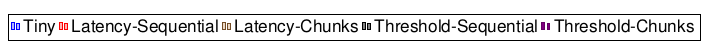
\includegraphics[scale=0.3]{images/legend}
    
    \subfloat[Labyrinth]{
        \label{Labyrinth}
        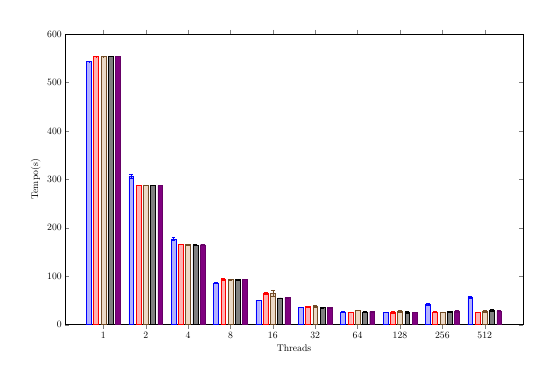
\begin{tikzpicture}[scale=0.35, baseline]
            \begin{axis}[
                width=1.5 \linewidth,
                height=1 \linewidth,
                %media de tempo intruder
                ybar=2.5pt,
                %enlargelimits=0.10,
                % legend style={at={(0.45,1.1)}, anchor=south, legend columns=-1},
                ylabel=Tempo(s),
                xlabel=Threads,
                symbolic x coords={1, 2, 4, 8, 16, 32, 64, 128, 256, 512},
                xtick=data,
                ymin=0,
                ymax=600,
                bar width=5pt,
                % nodes near coords,
                nodes near coords align={vertical},
            ]
            \addplot+[error bars,y dir=both, y explicit] coordinates {
                (1,543.12)+-(1,0.14) (2,307.12)+-(2,3.77) (4,177.18)+-(4,3.79) (8,86.06)+-(8,0.82) (16,50.63)+-(16,0.60) (32,35.89)+-(32,0.53) (64,26.45)+-(64,0.63) (128,25.83)+-(128,0.64) (256,41.98)+-(256,1.85) (512,57.32)+-(512,2.08) 
            };
            \addplot+[error bars,y dir=both, y explicit] coordinates {
                (1,553.57)+-(1,0.26) (2,287.70)+-(2,0.17) (4,165.86)+-(4,0.67) (8,94.13)+-(8,1.50) (16,65.04)+-(16,2.20) (32,37.22)+-(32,1.17) (64,25.60)+-(64,1.00) (128,25.49)+-(128,1.49) (256,26.10)+-(256,1.15) (512,25.80)+-(512,0.75)
            };
            \addplot+[error bars,y dir=both, y explicit] coordinates {
                (1,553.49)+-(1,0.21)(2,287.57)+-(2,0.25)(4,165.74)+-(4,0.99)(8,93.35)+-(8,1.29)(16,65.67)+-(16,6.11)(32,38.25)+-(32,1.76)(64,29.61)+-(64,0.77)(128,26.85)+-(128,2.24)(256,25.63)+-(256,0.42)(512,27.96)+-(512,1.35)
            };
            \addplot+[error bars,y dir=both, y explicit] coordinates {
                (1,553.89)+-(1,0.08) (2,287.30)+-(2,0.32) (4,164.88)+-(4,0.69) (8,93.33)+-(8,0.76) (16,55.06)+-(16,0.46) (32,35.27)+-(32,0.97) (64,26.35)+-(64,1.17) (128,26.33)+-(128,1.74) (256,26.96)+-(256,1.43) (512,29.70)+-(512,2.27) 
            };
            \addplot+[error bars,y dir=both, y explicit] coordinates {
                (1,553.38)+-(1,0.02) (2,287.58)+-(2,0.22) (4,164.99)+-(4,0.38) (8,93.83)+-(8,0.15) (16,55.92)+-(16,0.76) (32,35.17)+-(32,0.71) (64,26.79)+-(64,0.74) (128,25.67)+-(128,0.66) (256,27.99)+-(256,1.60) (512,28.01)+-(512,0.74)
            };
        % \legend {Tiny, Latency-Sequential, Latency-Chunks, Threshold-Sequential, Threshold-Chunks}
        \end{axis}
        \end{tikzpicture}
    }
    \subfloat[Vacation]{
        \label{Vacation}
        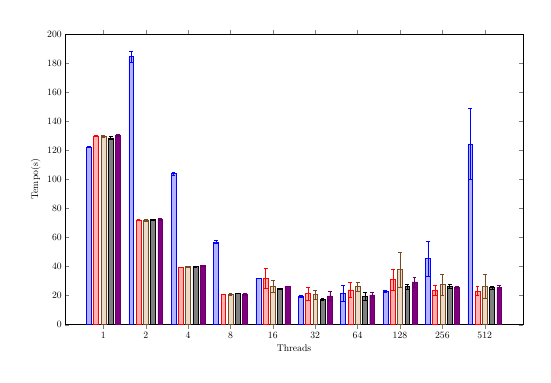
\begin{tikzpicture}[scale=0.35, baseline]
        \begin{axis}[
            width=1.5 \linewidth,
            height=1 \linewidth,
            %media de tempo intruder
            ybar=2.5pt,
            %enlargelimits=0.10,
            % legend style={at={(0.5,-0.15)}, anchor=north, legend columns=-1},
            ylabel=Tempo(s),
            xlabel=Threads,
            symbolic x coords={1, 2, 4, 8, 16, 32, 64, 128, 256, 512},
            xtick=data,
            ymin=0,
            ymax=200,
            bar width=5pt,
            % nodes near coords,
            nodes near coords align={vertical},
        ]
        \addplot+[error bars,y dir=both, y explicit] coordinates {
            (1,122.19)+-(1,0.35) (2,184.47)+-(2,3.93) (4,103.92)+-(4,1.04) (8,56.80)+-(8,1.07) (16,31.99)+-(16,0.24) (32,19.69)+-(32,0.52) (64,21.68)+-(64,5.72) (128,23.22)+-(128,0.57) (256,45.58)+-(256,11.99) (512,124.45)+-(512,24.20) 
        };
        \addplot+[error bars,y dir=both, y explicit] coordinates {
            (1,129.87)+-(1,0.52) (2,72.20)+-(2,0.44) (4,39.59)+-(4,0.19) (8,21.14)+-(8,0.09) (16,31.78)+-(16,6.87) (32,21.39)+-(32,4.41) (64,24.02)+-(64,4.93) (128,31.01)+-(128,7.24) (256,23.53)+-(256,3.50) (512,23.21)+-(512,3.03)
        };
        \addplot+[error bars,y dir=both, y explicit] coordinates {
            (1,129.58)+-(1,0.88) (2,71.87)+-(2,0.48) (4,39.90)+-(4,0.39) (8,21.15)+-(8,0.64) (16,26.35)+-(16,4.18) (32,20.69)+-(32,3.15) (64,26.17)+-(64,3.04) (128,38.12)+-(128,12.03) (256,27.50)+-(256,7.32) (512,26.48)+-(512,8.21)
        };
        \addplot+[error bars,y dir=both, y explicit] coordinates {
            (1,128.56)+-(1,0.95) (2,72.45)+-(2,0.41) (4,40.00)+-(4,0.22) (8,21.55)+-(8,0.22) (16,24.76)+-(16,0.20) (32,17.51)+-(32,0.39) (64,19.62)+-(64,2.71) (128,26.34)+-(128,1.81) (256,26.30)+-(256,1.52) (512,25.59)+-(512,1.05) 
        };
        \addplot+[error bars,y dir=both, y explicit] coordinates {
            (1,130.29)+-(1,0.63) (2,72.49)+-(2,0.59) (4,40.83)+-(4,0.31) (8,21.11)+-(8,0.63) (16,26.56)+-(16,0.15) (32,19.76)+-(32,3.23) (64,20.45)+-(64,1.74) (128,29.49)+-(128,3.46) (256,25.76)+-(256,0.95) (512,25.70)+-(512,1.49)
        };
        % \legend {Tiny, Latency-Sequential, Latency-Chunks, Threshold-Sequential, Threshold-Chunks}
        \end{axis}
        \end{tikzpicture}
    }
\end{figure}
